\documentclass[12pt]{article}
\usepackage[utf8]{inputenc}
\usepackage[T1]{fontenc}
\usepackage[a4paper,left=2cm,right=2cm,top=2cm,bottom=2cm]{geometry}
\usepackage[frenchb]{babel}
\usepackage{libertine}
\usepackage[pdftex]{graphicx}

\setlength{\parindent}{0cm}
\setlength{\parskip}{1ex plus 0.5ex minus 0.2ex}
\newcommand{\hsp}{\hspace{20pt}}
\newcommand{\HRule}{\rule{\linewidth}{0.5mm}}
\def\tab{$\>\>\>\>$}

% insérer une image en fixant la largeur = 0.5 * largeur du document pdf
\newcommand\img[2]{
\begin{figure}[!h]
  \centering
    \includegraphics[width=0.5\paperwidth]{#1}
  \caption{#2}
  \label{img:#1}
\end{figure}
}
%il faut l'utiliser comme ça : \img{image.extension}{légende}
%Pour la citer, utilier \ref{img:image.extension}

\begin{document}
\begin{titlepage}
  \begin{sffamily}
  \begin{center}

    % Upper part of the page. The '~' is needed because \\
    % only works if a paragraph has started.
    
\includegraphics[scale=0.2]{Images/Sorbonne_U.png}~\\[1cm] % mettre le logo de Sorbonne U à la place

    %\textsc{\LARGE Sorbonne Université}\\[1cm]

    \textsc{\Large Licence d'informatique}\\[1.5cm]

    % Title
    \HRule \\[1cm]
    { \huge \bfseries Projet Robotique\\[0.4cm] }

    \HRule \\[1cm]
    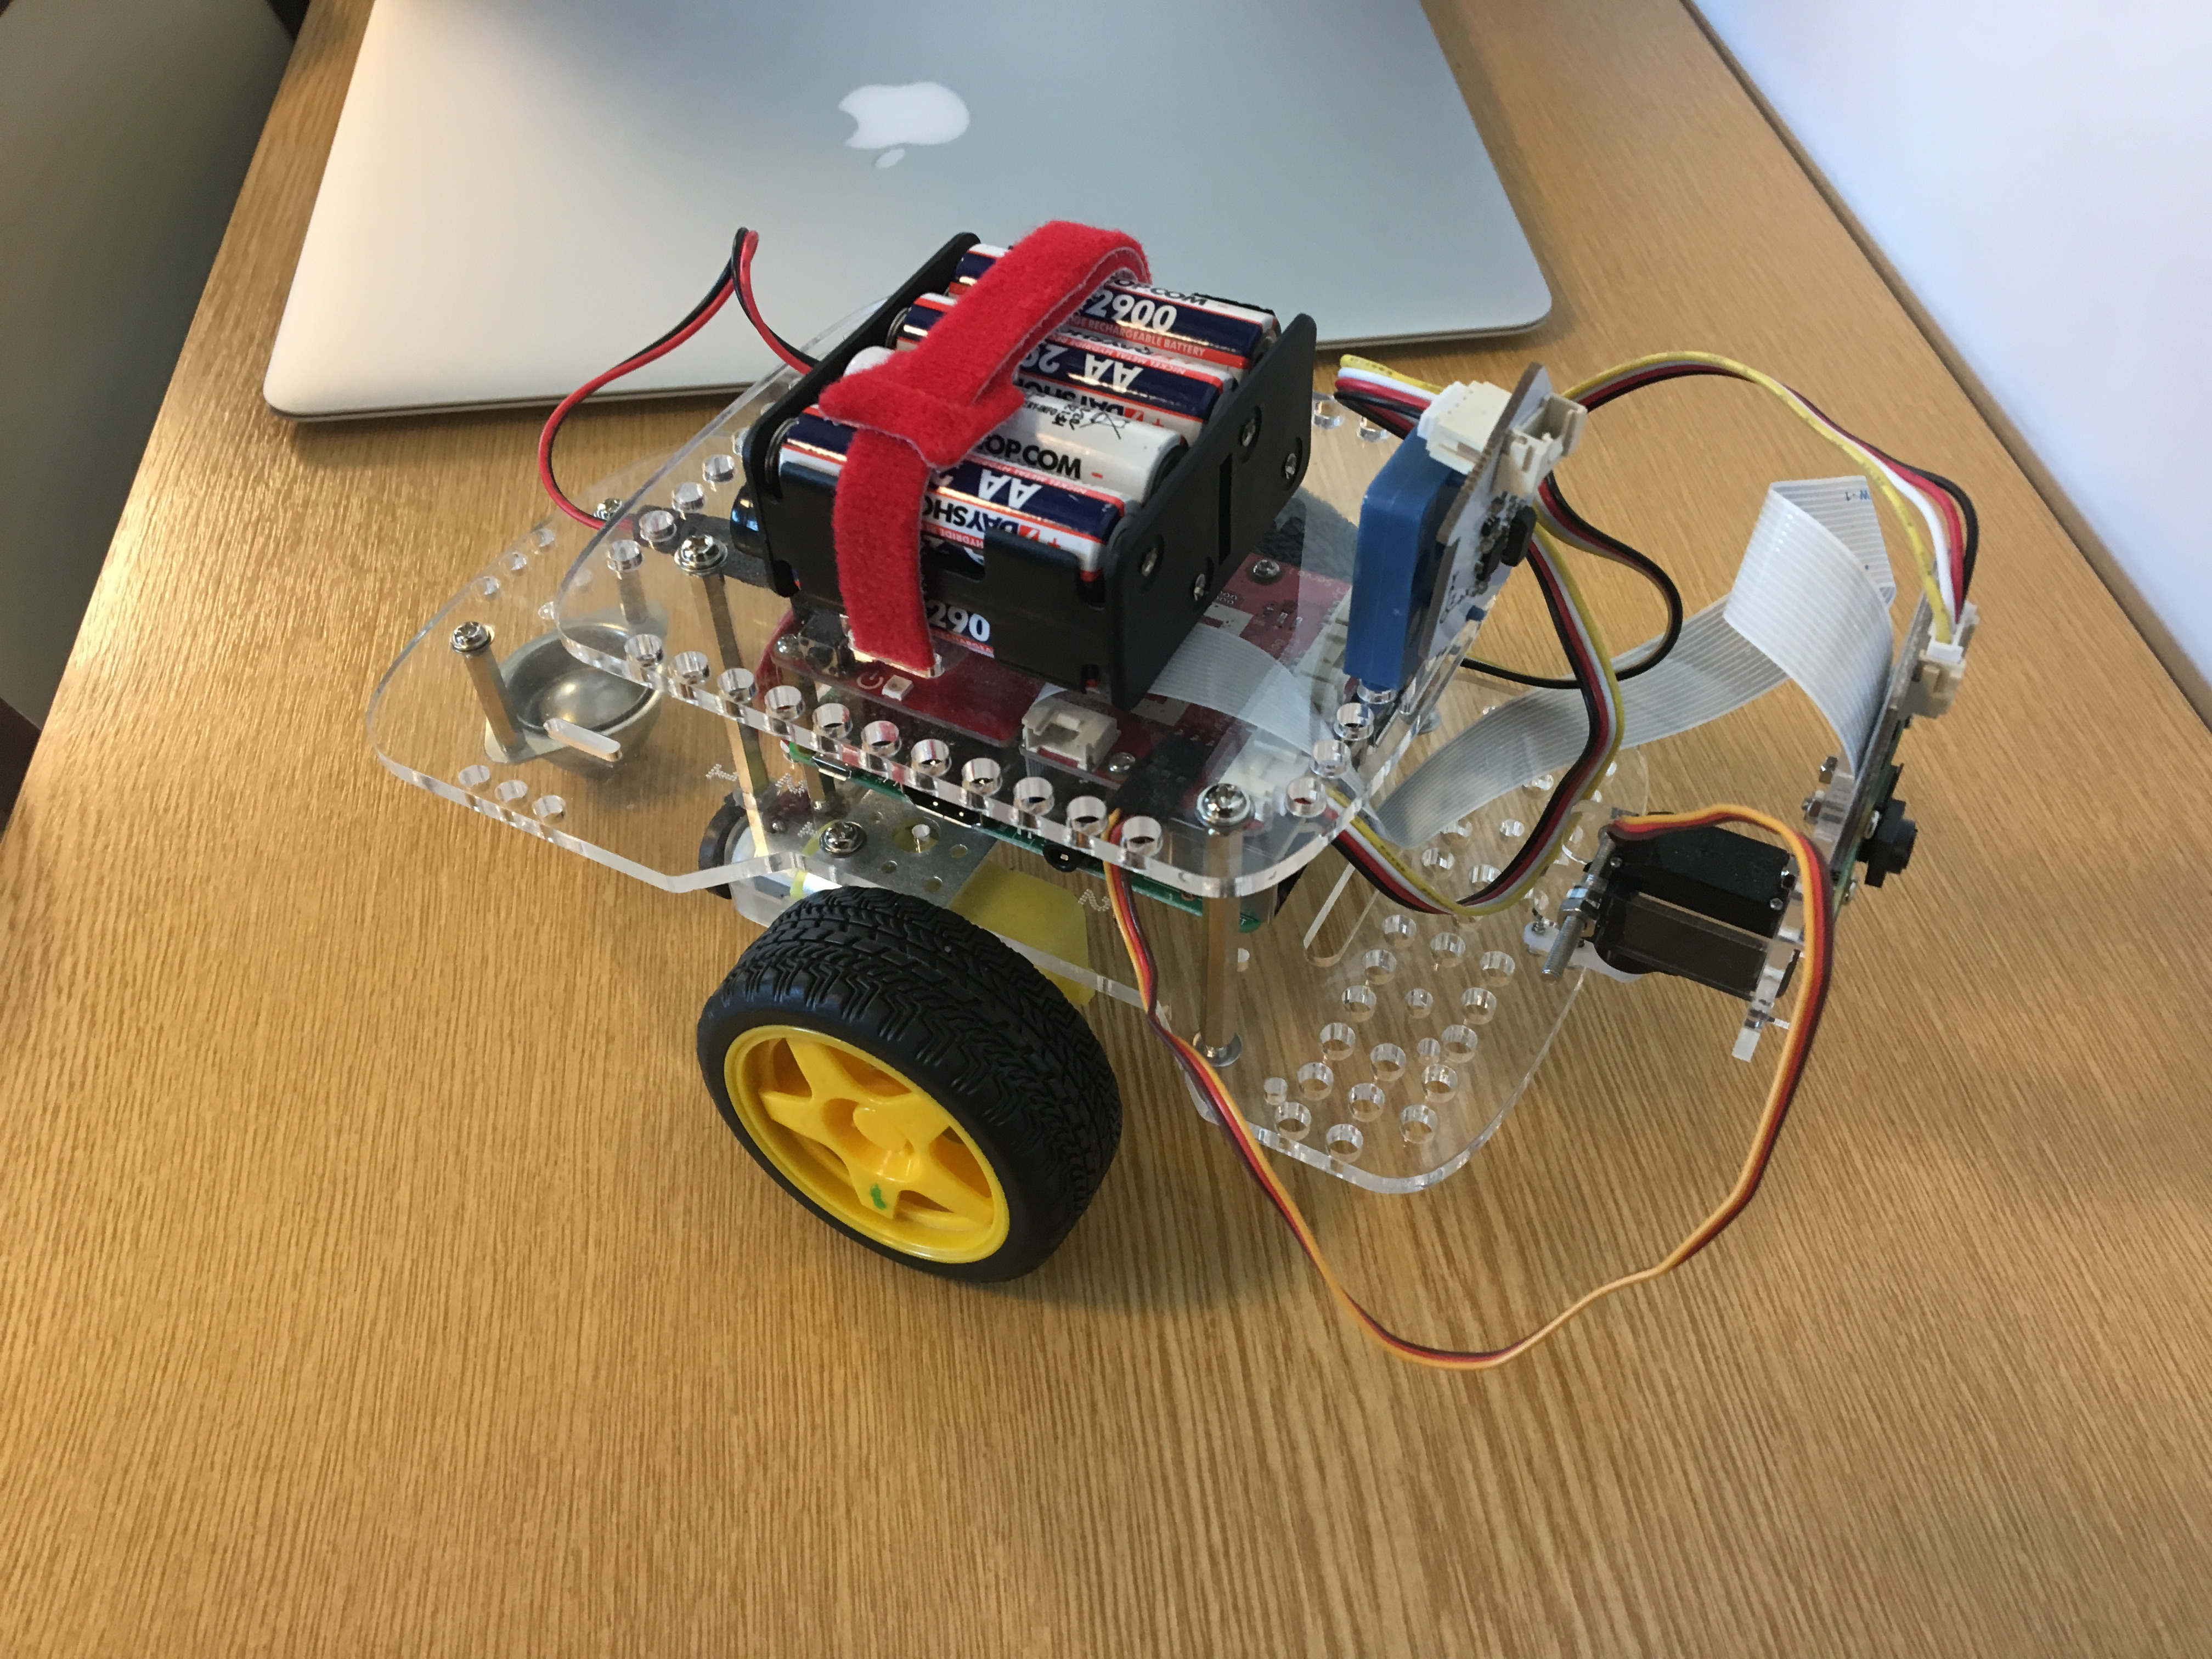
\includegraphics[scale=0.1]{Images/IMG_8579.JPG}
    \\[2cm]

    % Author and supervisor
    \begin{minipage}{0.4\textwidth}
      \begin{flushleft} \large
        Groupe \textsc{FiveGuys}\\
        UE 2I013\\
      \end{flushleft}
    \end{minipage}
    \begin{minipage}{0.4\textwidth}
      \begin{flushright} \large
        \emph{Chargé de cours:} M. \textsc{Baskiotis}\\
        \emph{Chargé de TME:} M. \textsc{Veniat}
      \end{flushright}
    \end{minipage}

    \vfill

    % Bottom of the page
    {\large 1\ier{} Février 2019 — Mai 2019}

  \end{center}
  \end{sffamily}
\end{titlepage}

\tableofcontents
\newpage
\section{Introduction}

\tab Dans le cadre de l'UE 2I013, notre projet était de concevoir un logiciel permettant de contrôler un robot ainsi que son simulateur. Nous avions en charge la totalité du projet et aucun code ne nous était fourni. Nos encadrants étaient à la fois nos superviseurs et nos clients. Il s'agissait donc d'échanger avec eux au sujet des éléments à changer et de l'avancement de notre projet.\\

\tab Les deux objectifs principaux de ce travail étaient : \begin{itemize}
\item[-] la découverte d'un projet de robotique
\item[-] la découverte des méthodes de travail en équipe
\item[]
\end{itemize}
\tab Le projet s'est développé en trois grandes étapes :\begin{itemize}
\item[-] dans un premier temps, il a fallu mettre en place les outils et méthodes nécessaires à notre travail d'équipe
\item[-] dans un deuxième temps, nous avons mis en place les briques de bases de notre projet tel que notre modèle physique ou notre simulateur 2D.
\item[-] pour finir, nous avons commencé à développer les stratégies qui nous permettent de répondre aux challenges qui nous on été soumis.
\end{itemize}


\newpage
\section{Rapport}
\subsection{Méthodes et outils}
\subsubsection{Agile/Scrum}

\tab Notre travail ne s'inscrivait pas seulement dans le cadre d'un projet de robotique, il avait également pour but de nous faire découvrir les méthodes de développement en équipe.

\tab En effet, dans les projets que nous réalisions jusqu'alors, nous ne nous occcupions pas particulièrement de la façon dont nous allions gérer le développement de nos projets. Les codes à développer sur quelques semaines seulement, en binôme ou trinôme, étaient relativement courts et guidés. Dans la plupart des cas, nous avions eu à réaliser des projets pour obtenir directement notre rendu final avec une méthode dite "en V". Cette dernière consiste en un développement du projet de A à Z à partir des exigences du "cahier des charges" (sujet) afin d'obtenir notre application. Les "retours client" se font donc en fin du développement. Il n'y a par conséquent aucune adaptation aux nouvelles exigences du client en cours de projet et les modifications à la fin de celui-ci sont rendues compliquées. Dans nos anciens projets cela ne posait pas problème mais dans le cadre de ce projet oui.

\tab Ce projet était construit de manière à ce que nous développions la totalité du code sur tout le semestre. Il nous fallait donc avoir un retour régulier sur l'avancement afin d'apporter des modifications et de s'adapter aux nouvelles exigences. Pour répondre à cette exigence, nous avons appliqué la méthode "Agile/Scrum", présentée en cours.

\img{Images/VueGlobaleScrum.png}{Schéma méthode Agile/Scrum}

\tab Cette méthode consiste à élaborer un ensemble de tâches. Ces dernières doivent être les plus petites et indépendantes possibles les unes des autres, et aisni forment ce que l'on appelle le "backlog". Les tâches doivent toutes être définies avec un maximum de précisions et en concertation avec toute l'équipe pour qu'il n'y ait pas de différence de résultat en fonction du membre du groupe qui l'accomplit. L'objectif, à l'issue du "sprint", est de réaliser une démonstration concrète des nouvelles fonctionnalités du projet.

\tab A l'issue de la nouvelle démonstration, les retours clients et le compte-rendu d'équipe rédigé permet de mettre en place le "backlog" et préparer le nouveau sprint.

\newpage

\subsubsection{Outils pour le travail d'équipe}
\paragraph{Git \& GitHub\\}
La logiciel de gestion de version Git, nous a permis de concerver une version centralisée du code. Ce système nous permet alors de développer un même code sans avoir à le partager manuellement à chaque modification. De plus, cette organisation, par la centralisation du code permet d'éviter un maximum de conflit lors du développement de celui-ci mais également de concerver une trâce de ses versions précédentes.

\paragraph{Trello\\}
\tab Pour mettre en place les différentes tâches présentes dans le backlog, nous avons utilisé le logiciel Trello. La fontionnalité de celui-ci permet de créer un tableau numérique qui facilite la mise en place de nos différentes tâches et leurs lisibilités. Dans un premier temps l'élaboration de nos sprints et la préparation de nos cartes nous on montrer une mauvaise mise en place d'Agile, ce qui nous a conduit comprhension des résultats attendus et parfois du travail en double.

\tab Par la suite, grace aux premières réunions et aux premiers retours, nous avons pu améliorer la préparations de nos sprints, et nous permettre ainsi d'avancer dans la préparation de notre simulateur avec une première interface et la mise en place de notre modèle.


\subsubsection{Hiérarchie du code}

\paragraph{MVC (\textit{Model-View-Controler})\\}
\tab La hiérarchie du code présenté ci-dessous se base sur une volonté d'appliquer un modèle de conception de logiciel (\textit{design pattern}) appelé le modèle \textit{MVC} (Modèle - Vue - Contrôleur). Ce \textit{design pattern} impose une hiérarchie du code très précise qui comprend trois parties distinctes : \begin{itemize}
\item[-] la partie modèle gère les données relatives au programme mais également les calculs sur celles-ci,
\item[-] la partie contrôleur fait le lien entre l'affichage et le modèle, le contrôleur transmet à la vue les données à afficher depuis le modèle et communique en retour les informations issues des interactions avec l'interface au modèle,
\item[-] la partie vue gère uniquement l'affichage à partir des informations qui lui sont communiquées par le contrôleur.
\end{itemize}

\newpage
\paragraph{\\}

\begin{figure}[!h]
  \centering
    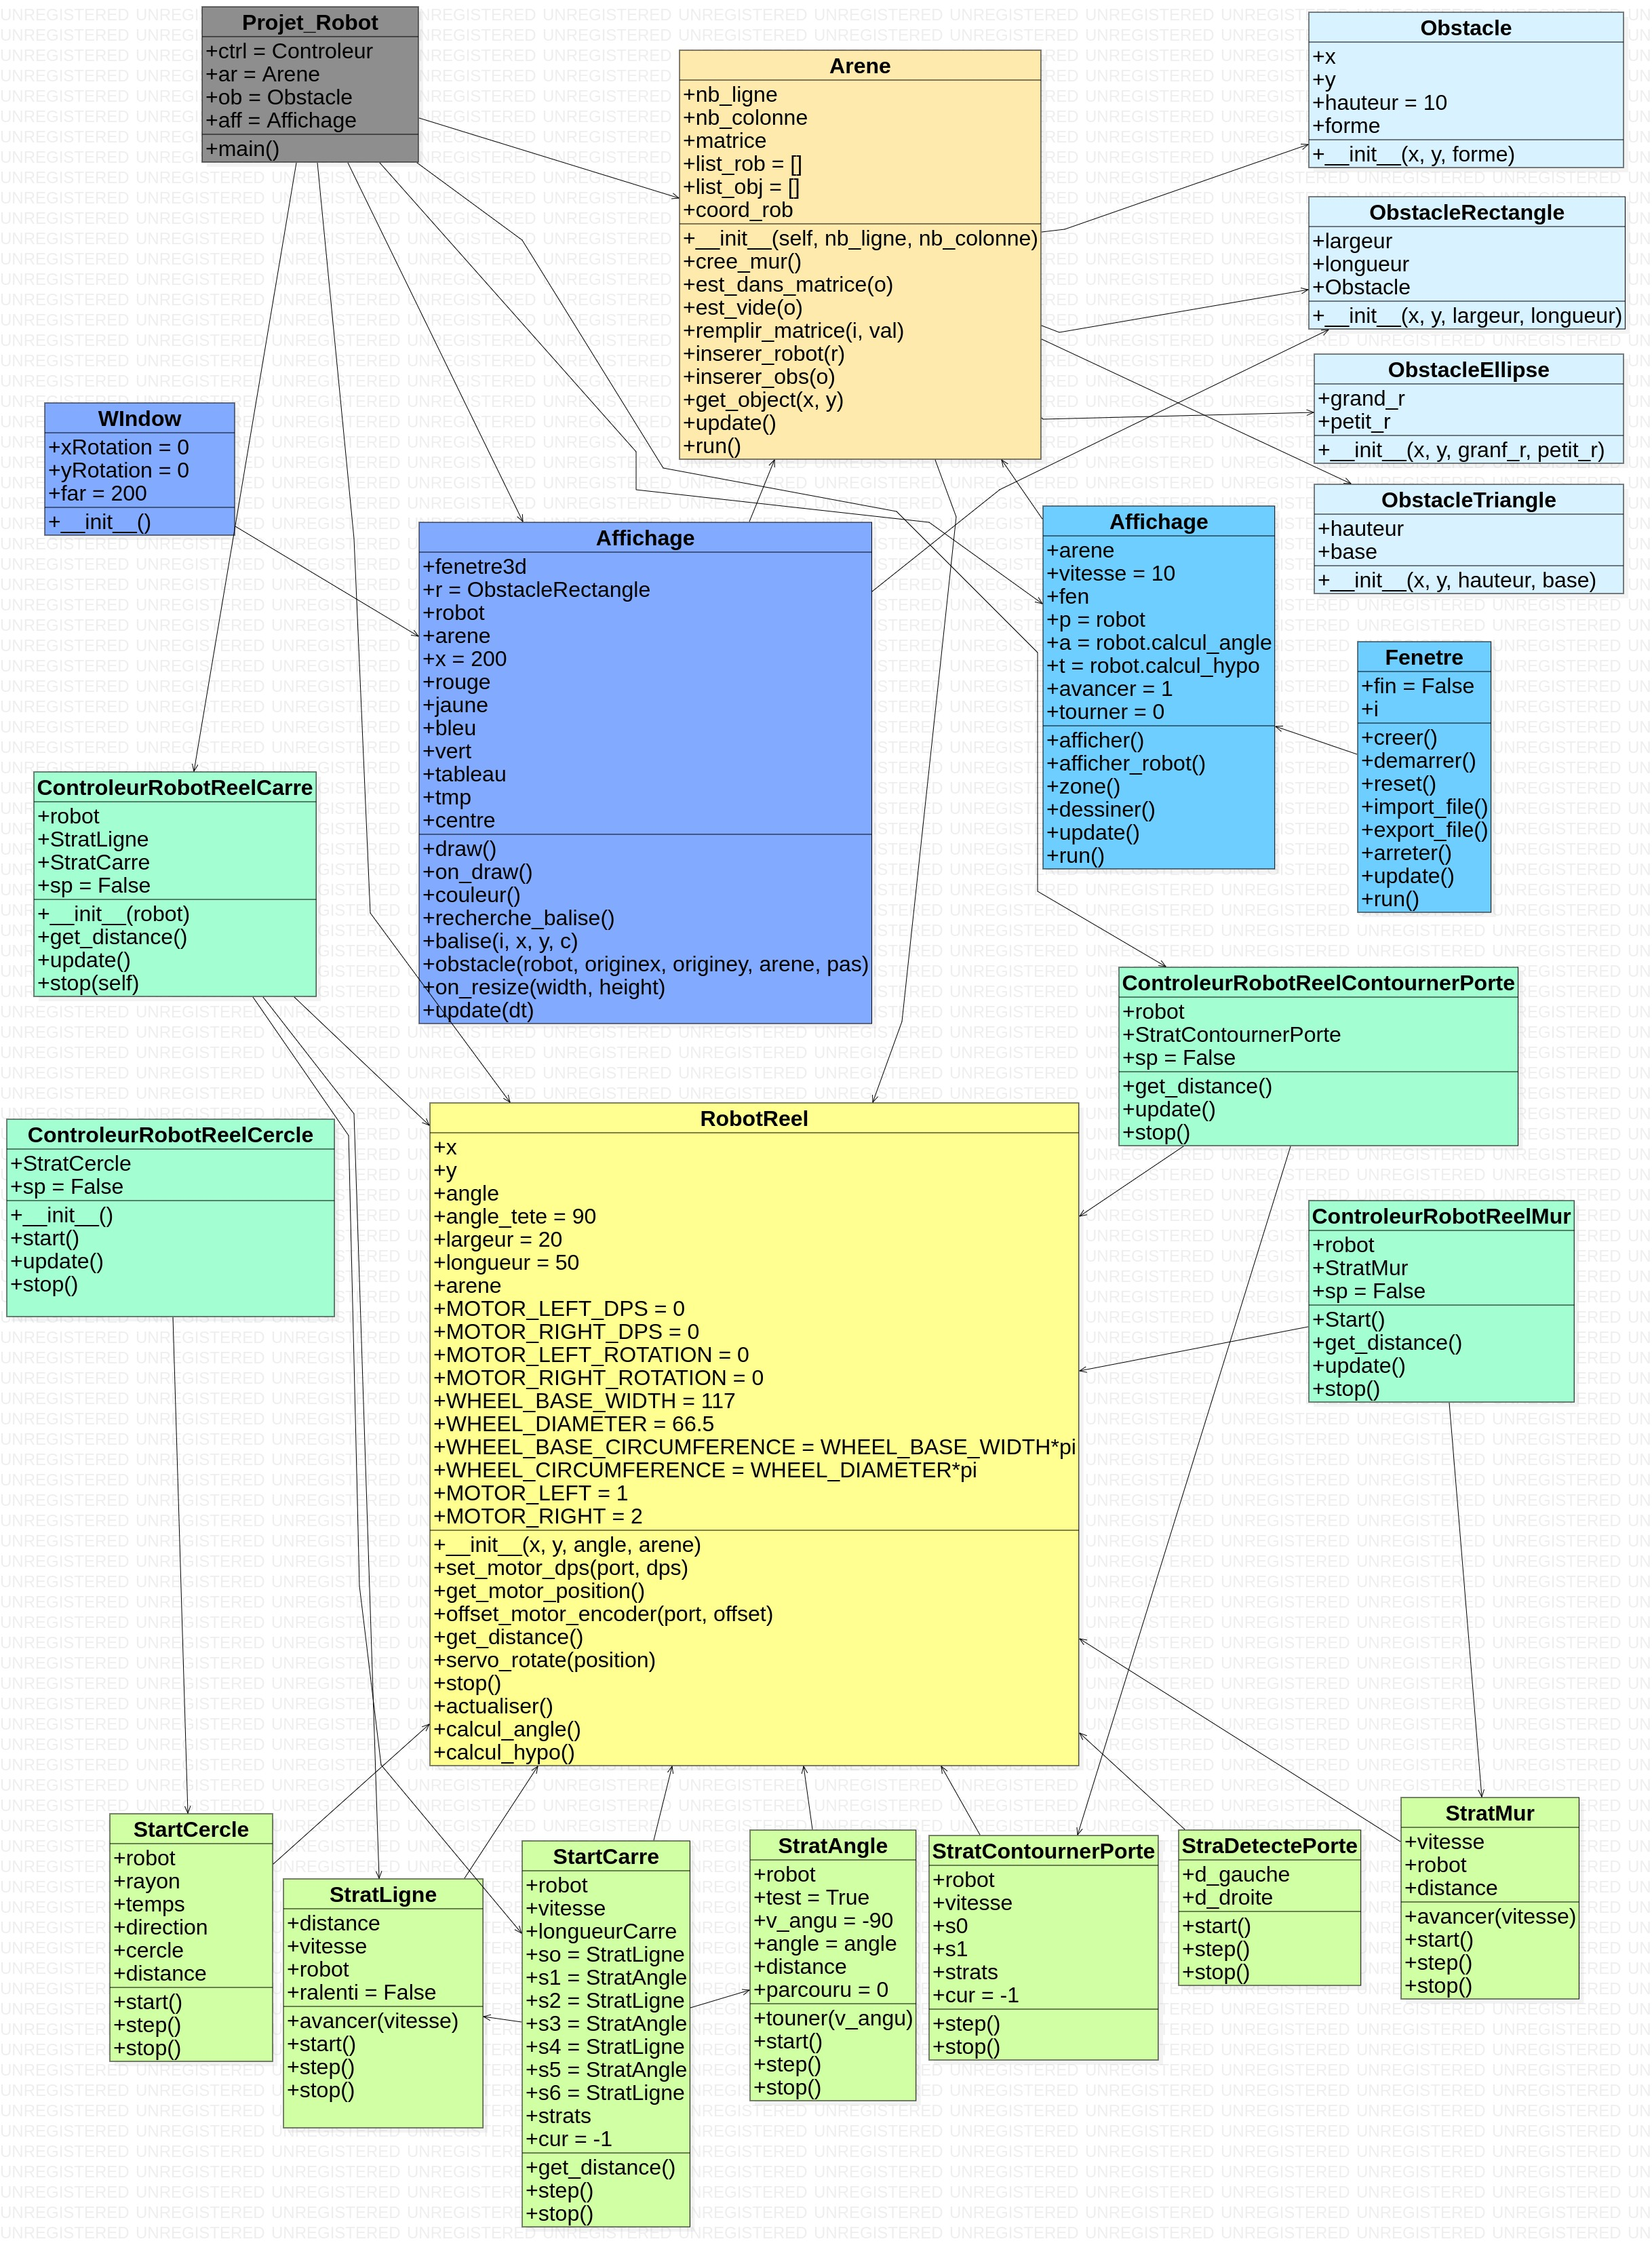
\includegraphics[width=0.80\paperwidth]{Images/ProjetRobotique6.jpg}
  \caption{Hiérarchie du code}
  \label{img:Images/ProjetRobotique6.jpg}
\end{figure}

%\newpage
\subsection{Mise en place de briques de base}
\subsubsection{Modélisation du réel}
\tab Comme nous le savons, le but du projet est de modéliser les différents comportements d’un robot dans son environnement. Autrement dit, le déplacement d’un robot dans une arène semée d’obstacles. Nous remarquons ainsi la présence des termes de nos objets de bases: une arène, un robot et des obstacles.
\paragraph{Notre Arène\\}
Le terme d’arène peut être vulgarisé par le terme d’espace. C’est l’environnement dans lequel nous allons conserver nos données. Quoi de mieux qu’une matrice ? Une matrice $M \times N$ est un tableau de nombres à M lignes et N colonnes. Les nombres présents dans la matrice sont appelés « éléments de la matrice ».  Ce type de tableau va nous permettre de différencier les objets présents ainsi que leurs coordonnées. Par exemple, nous avons de décidé d’attribuer le chiffre, « 0 » aux emplacements vides, « 1 » au centre de notre robot et « 2 » aux zones occupées par des obstacles. Pour résumer, grâce à cette perspective nous pouvons savoir où se trouve notre robot et si un objet est présent à la colonne x et à la ligne y.
\paragraph{Notre Robot\\}
Nous avons décidé de modéliser notre robot comme un rectangle muni d’un angle de direction car ce sont les concepts de base se rapprochant au maximum de nos contraintes dans notre contexte. Son corps est ainsi un rectangle (rouge) muni d’une certaine longueur et d’une certaine largeur. Si nous voulons savoir où se trouve notre robot, nous avons qu’à parcourir la matrice et chercher l’élément ayant pour valeur « 1 ». Cependant, cela ne correspond qu’au centre du robot et non l’espace total qu’il occupe. Nous savons que notre robot possède un centre de coordonnées [ x , y ], une longueur et une largeur. Ainsi, l’espace occupé est réellement tous les éléments de l’arène ayant une abscisse comprise entre ‘ ’x – largeur /2 ’’ et ‘’x + largeur/2’’ et une ordonnée comprise entre ‘ ’y – longueur /2 ’’ et ‘’y + longueur/2’’. Pour mieux visualiser, vous trouverez un schéma ci-dessous :

\img{Images/Robot.png}{Modélisation de notre arène}

\paragraph{Nos Obstacles\\}
Dans la même idée que pour notre robot, nos obstacles sont modélisés par des rectangles noirs, avec une longueur et une largeur. Dans notre matrice, leur centre correspondent aux éléments « 2 ». Les différencier par la valeur de leurs éléments va nous permettre de connaître, par exemple, leur nombre, leurs coordonnées et l’espace qu’ils occupent individuellement. Cela va nous être très utile pour transmettre à notre robot quelles zones il doit contourner.

\subsubsection{Mise en place de l'interface graphique 2D}
Nous avons à notre disposition différentes classes comme Robot, Arène et Obstacle. Cependant,  cela n’est que du code et nos clients ne sont pas forcément experts en informatique. Nous devions trouver un moyen adapté pour favoriser la compréhension de notre avancement dans le projet. Voilà pourquoi une grande partie de notre travail était de modéliser l’attente de notre client sous forme de simulation 2D.

\paragraph{Tkinter\\}
Après de nombreuses recherches, nous avons fini par trouver le module Python spécifique aux interfaces graphique 2D qui nous convenait le mieux : Tkinter. Il est adapté à chaque OS, fourni avec Python et compatible avec Python 3. Ainsi, après la conception de notre Modèle (ensemble des classes Arène, Robot et Obstacle), nous pouvons nous concentrer sur notre Affichage.
Grâce à Tkinter, nous pouvons ainsi créer une fenêtre affichant le robot et les obstacles. De plus, nous y avons ajouté des évènements permettant ainsi aux clients d’interagir avec son robot (hors démo) ou encore des boutons permettant l’importation et l’exportation de différentes simulations.
Vous trouverez ci-dessous différentes captures d’écran imageant quelques situations :

\subsubsection{Stratégies de base}
\paragraph{Ligne droite\\}
Notre premier objectif a été de faire avancer notre robot en ligne droite. Pour cela, nous réalisions une modification des coordonnées du robot pour le déplacer d'une distance fournie en argument. Pour le faire avancer en ligne droite selon son orientation, nous avons au robot un paramètre d'angle qui indique à tout moment son orientation sur le cercle trigonométrique. Ainsi, les fonctions trigonométriques nous permettaient de facilement coefficienter la modification des paramètres, et donc de le faire se déplacer dans la bonne direction.

\paragraph{Rotation\\}
Le second objectif a été de déterminer comment faire tourner le robot. La méthode la plus simple était de le faire tourner sur lui-même, n'ayant pas à gérer de modification de ses coordonnées. L'implémentation du paramètre d'angle a grandement facilité la réalisation de cette fonction, puisque réduite a une modification de paramètre.

\paragraph{Detection d'obstacles\\}
Le robot étant doté d'un capteur permettant de déterminer sa distance à un obstacle devant lui, il nous fallait inclure cette fonctionnalité à notre robot simulé. Pour cela nous avons implémenté un capteur, qui au lancement de la fonction se déplace en ligne droite en partant du robot d'un pas fourni en argument, et selon la même procédure de calcul que pour de déplacement du robot. A chaque pas, le capteur observe la valeur de la matrice sur ses coordonées. S'il détecte un "0", il continue à avancer, s'il rencontre un "2" (un obstacle), il s'arrête et la fonction renvoie les dernières coordonnées du capteur, qui étaient ensuite interprétées pour calculer la distance à l'obstacle.

\subsubsection{Passage de la simulation au réel}
\tab L'une des exigences pour projet était que notre code ne devait pas dépendre du fait que celui-ci soit lancé dans notre simulateur ou dans notre robot. Le but étant de pouvoir tester les nouvelles fonctionnalitées de notre robot, nous voulions les ajouter comme si elles étaient déjà dans le robot. Ainsi l'implémentation dans le robot peut être directe et normalement sans bug. La démarche que nous devions adopter nous permet ainsi également de pas développer le code en double.

\tab Nous avons donc du réadapter notre code afin de pouvoir répondre à cette contrainte. Notre première version du robot mise en place dans le simulateur ne répondait pas à cette attente. En effet, il n'était pas conçu de tel sorte qu'il puisse répondre au instructions de la véritable API du robot. Nous avons donc dans un premier temps créé un nouveau robot, fonctionnant dans notre simulation comme le premier robot, mais ne réagissant qu'aux fonctions de l'API du robot. Cette nécessité de créer un nouveau robot à été dans un premier temps problématique car il nous fallait complétement repenser notre robot. Une fois la solution trouvée nous avons pu avancer dans la mise en place des briques de base et le perfectionnement de notre simulateur.

\tab Dorénavant, le code sera indifférencié qu'il soit utilisé dans le robot ou dans le simulateur. Mais alors comment faire la différence ? La différence se fait au moment du lancement de notre script, en jouant sur l'importation de l'API intégré à notre robot. Si python réussi à importer l'API alors on est dans le véritable robot sinon nous sommes dans notre simulateur.
%Dans un premier temps nous avons donc rajouté une surcouche au niveau de notre robot afin que les fonctions du robot de la simulation soit identiques aux fonctions de l'API du robot. Notre premier robot, telle qu'il est décrit plutôt. Nous avons redifini les paramètres afin qu'il soit ceux du robot. Cette surcouche au niveau du robot permet de faire la traduction pour le véritable robot.

\begin{center}
Ajout d'un petit schéma à propos du lancement des scripts
\end{center}

\newpage
\subsection{Développement des stratégies}
\subsubsection{Stratégie carré}
\tab Notre première grand objectif a été d'implémenter une stratégie carré. Pour ce faire nous avons utiliser les stratégies ligne et angle. Les paramètres de la stratégie carré sont le robot, sa vitesse et la longueur de carré a réalisé. Pour que le robot puis réaliser un carré il nous a fallu implémenter 4 stratégies ligne possèdant les mêmes paramètres, et 4 stratégies angle possèdant également les mêmes paramètres. Par la suite on ajoute chacune de ses stratégies dans un tableau, qui effectura le mouvement d'un carré. Notre stratégie va donc parcourir ce tableau, jusqu'à ce qu'il n'y est plus de stratégie, en affichant a chaque déplacement sa distance. Cependant, lors de notre premiers essai, nous n'avons pas obtenu un carré parfait car on obtenait un légère différence au niveau de la premier rotation, ce qui entrainait une modification sur les quatres côtés du robot. Ainsi, pour combler ce problème, nous avions penser a diminué la vitesse du robot sur les stratégies de base avant que le robot effectue une rotation, pour que chaque rotation du robot soit identique à la valeur que nous avions attribué dans les paramètres du robot.

\subsubsection{Stratégie détection de mur}
\tab La stratégie « détection de mur » est la stratégie répondant à l’une des missions confiées par nos clients. En effet, la mission consiste à modéliser la course du robot en ligne droite, fonçant dans un mur et s’arrêtant juste avant la collision.
Cependant, certaines contraintes s’imposent à nous : \begin{itemize}
\item[-] La trajectoire de la course du robot est perpendiculaire au mur. En effet, le capteur de distance permettant la détection d’obstacles est au centre de la face avant du robot. Si nous déviions le robot cela pourrait causer la collision entre le mur et le coin du robot.
\item[-] La distance entre la position initiale du robot et le mur vers lequel il se dirige ne doit pas dépasser 8,000 millimètres car cela correspond à la limite du capteur de distance.
\item[-] Il n’y a aucun obstacle entre le mur et le robot
\end{itemize}
La stratégie aura un attribut "distance" qui sera la distance entre lui et le mur et à laquelle le robot va devoir interrompre sa course.
Nous avons à notre disposition la méthode "get\_distance" qui nous renvoie la distance entre la face avant du robot et l’obstacle le plus proche si la valeur de retour est comprise entre 5 et 8,000 millimètres, sinon elle nous renvoie "8190". Ainsi, nous appelons cette méthode « en continu » et nous vérifions si la distance passée en paramètre est inférieure à la distance retournée par "get\_distance" ou si la valeur retournée est égale à 8190 car cela voudrait dire que le robot est à moins de 5 millimètre.
Ainsi, le robot va tout droit dans le mur, et si la distance est suffisamment petite il s’arrête.

\subsubsection{Stratégie cercle}
\subsubsection{Stratégie contourner une porte}
\tab La stratégie pour contourner la porte est une stratégie qui a pour but d'expérimenter une première stratégie qui ne soit pas complètement définie à l'avance. En effet, cette stratégie est construite de telle sorte que le robot puisse passer la porte qu'elle se trouve sur sa droite ou sur sa gauche. La stratégie en elle-même se déroule de la façon suivante : \begin{itemize}
\item[-] le robot se trouve face au mur de la porte et avance,
\item[-] une fois au mur on détecte le côté de la porte en tournant la tête du robot et en utilisant le capteur de distance,
\item[-] on tourne du cote de la porte qui se trouve à la distance la plus courte au niveau du retour du capteur,
\item[-] puis on se replace dans l'axe précedent
\item[-] on fini ensuite par traverser le couloir jusqu'au mur.
\end{itemize}
\tab Pour mettre en place cette stratégie, nous avons pris le parti de concidérer des portes s'ouvrant uniquement vers l'intérieur de la pièce et de façon perpendiculaire comme la porte de notre salle de TP. Ainsi le capteur de détecte la porte qui se trouve alors à la distance la plus courte et le robot tourne vers elle. Ce choix est arbitraire et peut causer quelque souci lors de l'utilisation si le mur si trouve plus pret du robot.

\subsubsection{Stratégie détection balise}
\paragraph{Nécessité d'une interface 3D \\}
\tab La mise en place de l'interface 3D était nécessaire pour la réalisation du challenge detection de balise car nous avions besoin de simuler la camera frontal du robot. Nous avons donc choisi le module pyglet comme préconisé dans le cour sur la 3D puis nous avons suivi différent tuto afin de maîtriser le dessin en 3D ainsi que le positionnement de la camera. L'implémentation de la 3D fut plus simple que celle de la 2D car nos différentes stratégies étaient déjà débuggés et fonctionnels .

\paragraph{Mise en place de la stratégie de détection\\}
\tab En ce qui concerne le fonctionnement de la stratégie, on commence par ouvrir l'image à analyser, puis on prend chaque pixel et on verifie sa couleur. Si sa couleur correspond à l'une des quatre (bleu,vert,jaune,rouge) visible sur la balise alors on verifie chaque pixel à sa droite à la recherche d'une des trois autres couleurs attendu. Si on en trouve une couleur attendu on cherche en bas l'une des deux restantes. Et pour finir si l'on a atteint la troisième couleur on recherche la dernière à gauche. La stratégie n'est pour le moment pas réelement fonctionnel. Du moins pas sur le robot réel dû à la difficulté de detecter des couleur sur une photo prise par celui-ci.

\img{Images/baliseschema.png}{Schéma détection balise}

\newpage

\section{Remerciements}

\newpage

\section{Conclusion}

\newpage

\section{Sources}

\end{document}
